\begin{figure}
	\begin{center}
	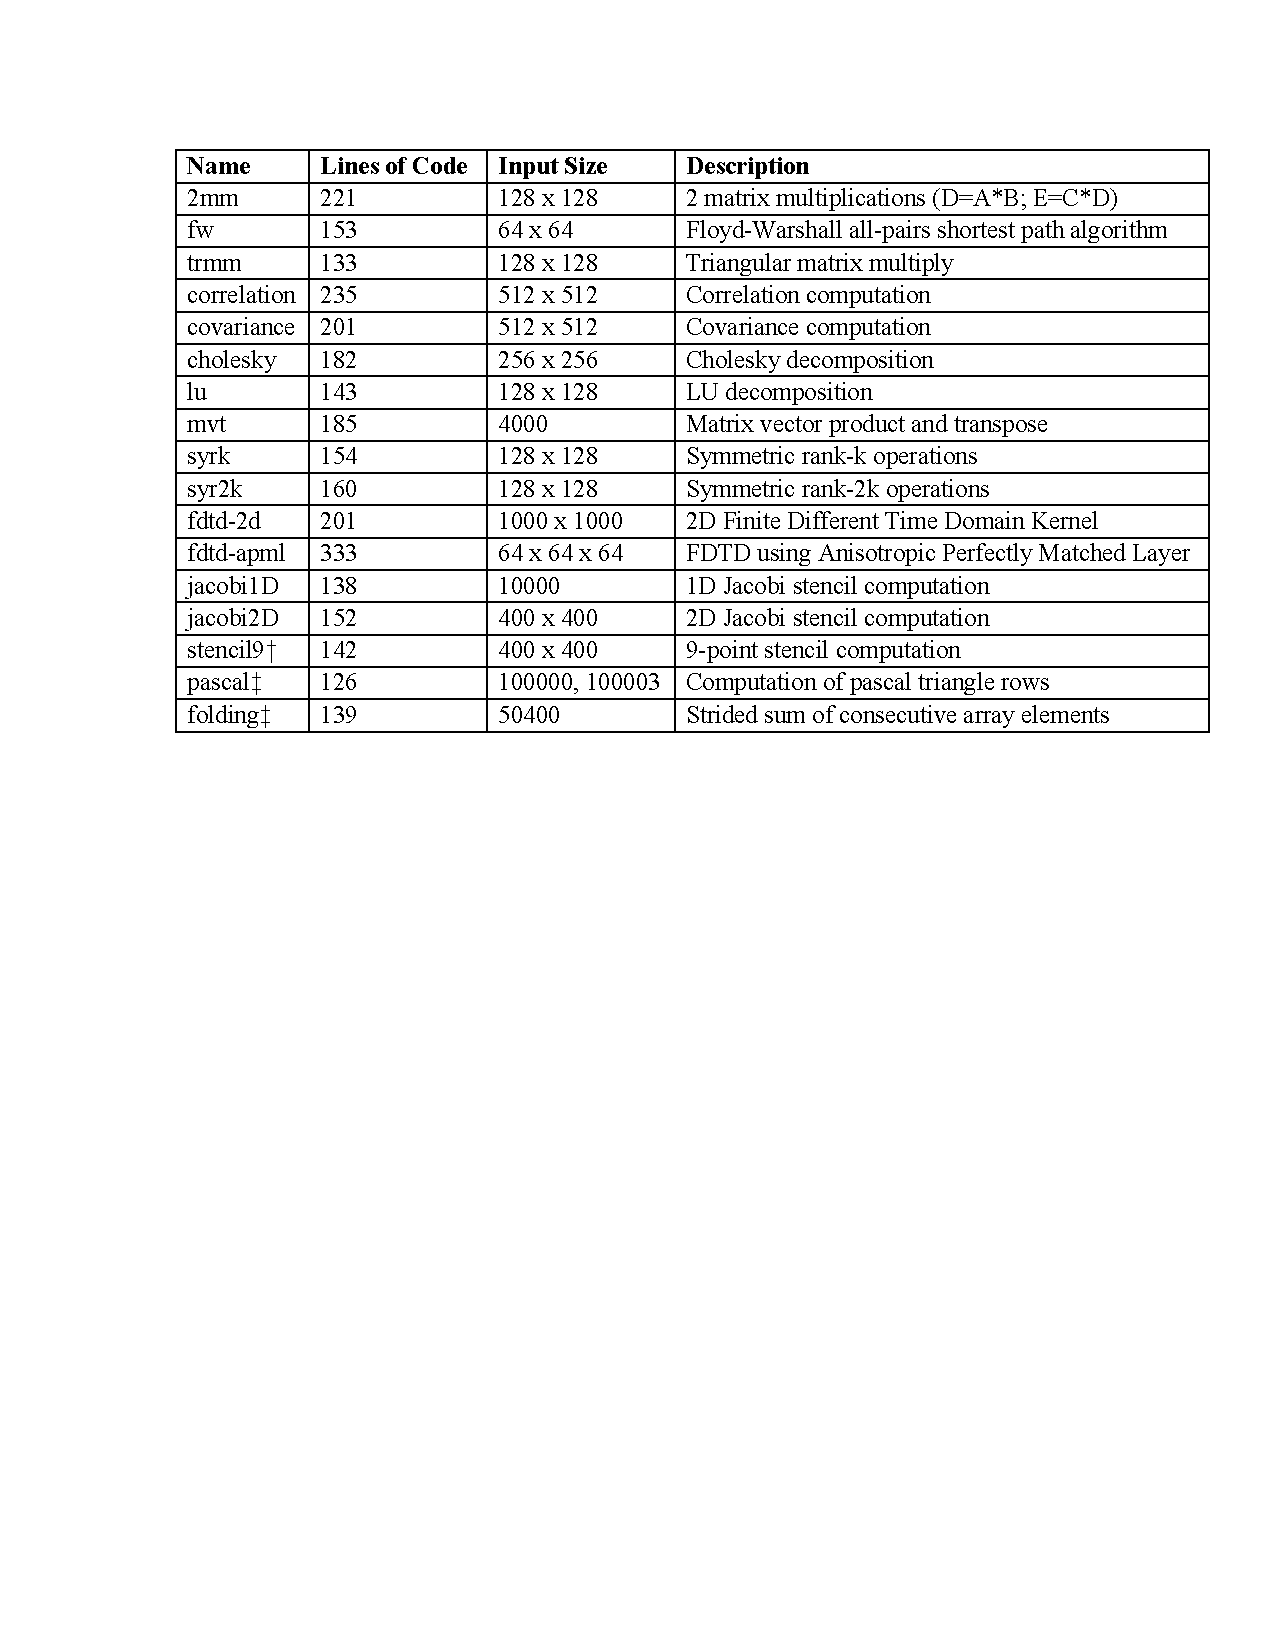
\includegraphics[scale=0.53]{./Figures/Benchmarks.pdf}
	\caption{Benchmark suite. Benchmarks with no symbol after their name were taken from the Polybench suite of benchmarks and translated to Chapel. Benchmarks with $\dagger$ are taken from the Chapel Trunk test directory. Benchmarks with $\ddagger$ were developed on our own in order to test specific data access patterns. }
	\label{benchmarks}
	\end{center}
\end{figure}

\section{Results}\label{sec:results}

To demonstrate the effectiveness of modulo unrolling WU in the Chapel Cyclic and Block Cyclic distributions, we present our results. We have composed a suite of seventeen parallel benchmarks shown in Figure \ref{benchmarks}. Each benchmark is written in Chapel and contains loops with affine array accesses that use zippered iterations, as discussed in \ref{sec:array_slicing}. Our suite of benchmarks contains programs with single, double, and triple nested affine loops. Additionally, our benchmark suite contains programs operating on one, two, and three-dimensional distributed arrays. Fourteen of the seventeen benchmarks are taken from the Polybench suite of benchmarks \cite{polybench} and are translated from C to Chapel by hand. The \textit{stencil9} benchmark was taken from the Chapel source trunk directory. The remaining two benchmarks, \textit{pascal} and \textit{folding}, were written by our group. \textit{pascal} is an additional benchmark other than \textit{jacobi1D} that is able to test Block Cyclic with modulo unrolling WU. \textit{folding} is the only benchmark in our suite that has strided affine array accesses. 

To evaluate improvements due to modulo unrolling WU, we run our benchmarks using the Cyclic and Block Cyclic distributions from the trunk revision 22919 of the Chapel compiler as well as the Cyclic and Block Cyclic distributions that have been modified to perform modulo unrolling WU, as described in Section \ref{sec:adaptation_in_chapel}. We measure both runtime and message count for each benchmark. We also compute the geometric means of all normalized runtimes and message count numbers for both distributions to get a sense on average of how much improvement modulo unrolling WU provided. Data was collected on the eight-locale Golgatha cluster at the Laboratory for Telecommunication Sciences in College Park, Maryland. 

When evaluating modulo unrolling WU used with the Block Cyclic distribution, we could only run two benchmarks out of our suite of seventeen because of limitations within the original Chapel Block Cyclic distribution. Many of our benchmarks operate on two or three-dimensional arrays and all require array slicing for the modulo unrolling WU optimization to apply. Both array slicing of multi-dimensional arrays and array slicing containing strides for one-dimensional arrays are not yet supported in the Chapel compiler's Block Cyclic distribution. Implementing such features remained outside the scope of this work. There was no limitation when evaluating modulo unrolling WU with the Cyclic distribution, and all seventeen benchmarks were tested. Once these missing features are implemented in the Chapel compiler, then our method will apply to all of our benchmarks.

\begin{figure}
	\begin{center}
	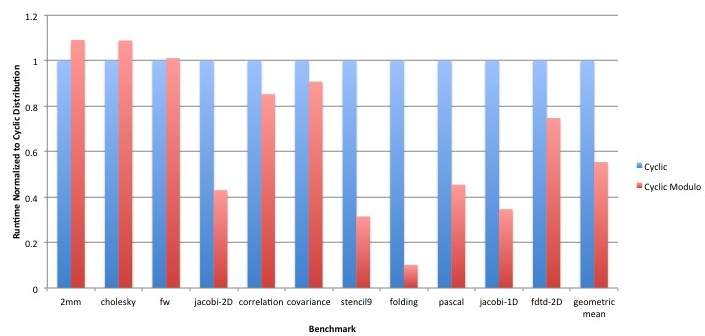
\includegraphics[scale=0.30]{./Figures/cyclic_runtime}
	\caption{Cyclic runtime.}
	\label{cyclic_runtime}
	\end{center}
\end{figure}

\begin{figure}
\begin{center}
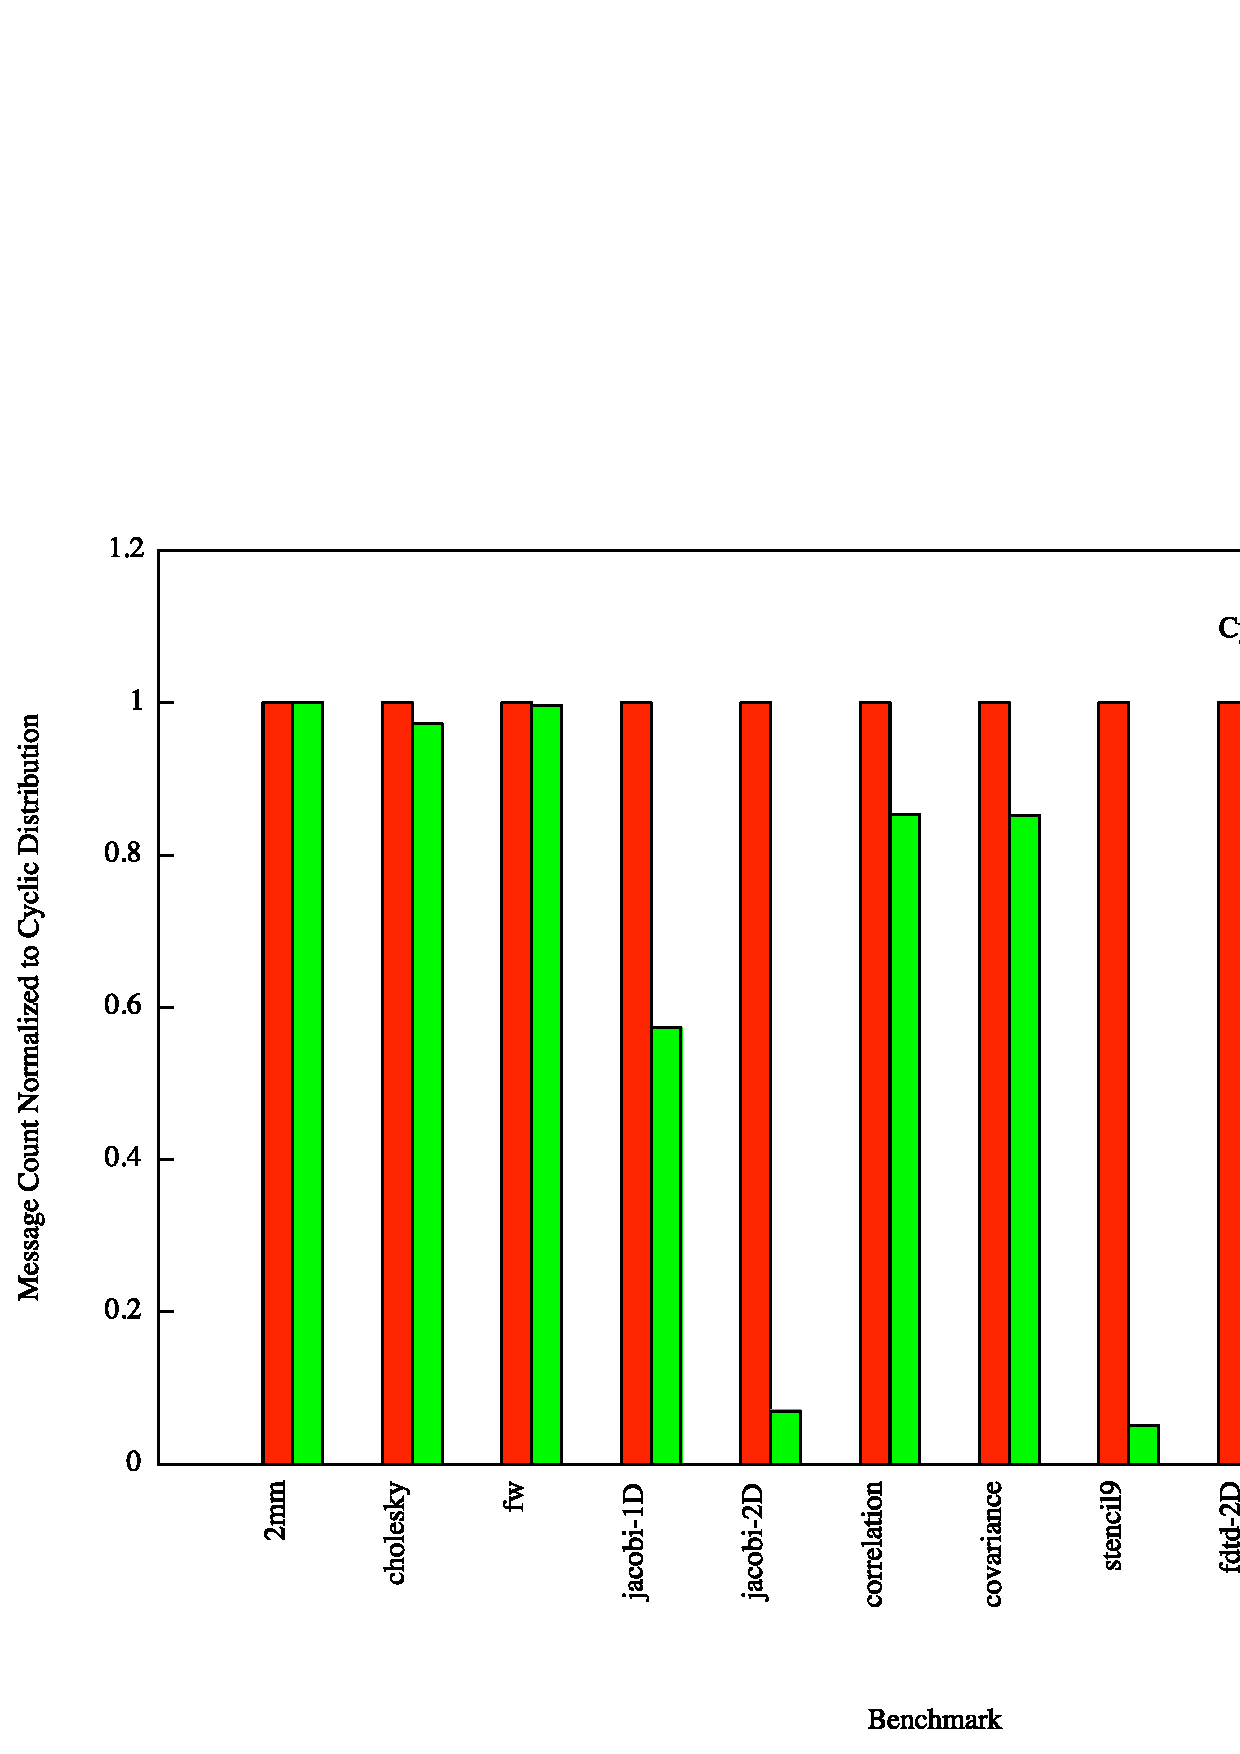
\includegraphics[scale=0.30]{./Figures/cyclic_message_count}
\caption{Cyclic message count.}
\label{cyclic_message_count}
\end{center}
\end{figure}

Figures \ref{cyclic_runtime} and \ref{cyclic_message_count} compare the normalized runtimes and message counts respectively for the Cyclic distribution and Cyclic distribution with modulo unrolling WU. For 8 of the 11 benchmarks, we see reductions in runtime when the modulo unrolling WU optimization is applied. On average, modulo unrolling WU results in a 45 percent decrease in runtime. For 9 of the 11 benchmarks, we see reductions in message counts when the modulo unrolling WU optimization is applied. On average, modulo unrolling WU results in 76 percent fewer messages. 

Some detailed observations on Figures \ref{cyclic_runtime} and \ref{cyclic_message_count} follow. Two of the benchmarks, \textit{cholesky} and \textit{fw}, showed slight improvements in message count when using modulo unrolling WU but did not show improvements in runtime. For the \textit{2mm} benchmark, both runtime and message count did not improve when using modulo unrolling WU. For these benchmarks, the ratio of the problem size to number of locales is not high enough, leading to an insufficient amount of aggregation possible for the computation to see performance improvements. An increase in the number of locales on a system leads to fewer data elements per locale, which naturally means fewer data elements can be aggregated. When this occurs, the cost of performing bulk transfers of a few data elements is more expensive than transferring elements individually. 

\begin{figure}
\begin{center}
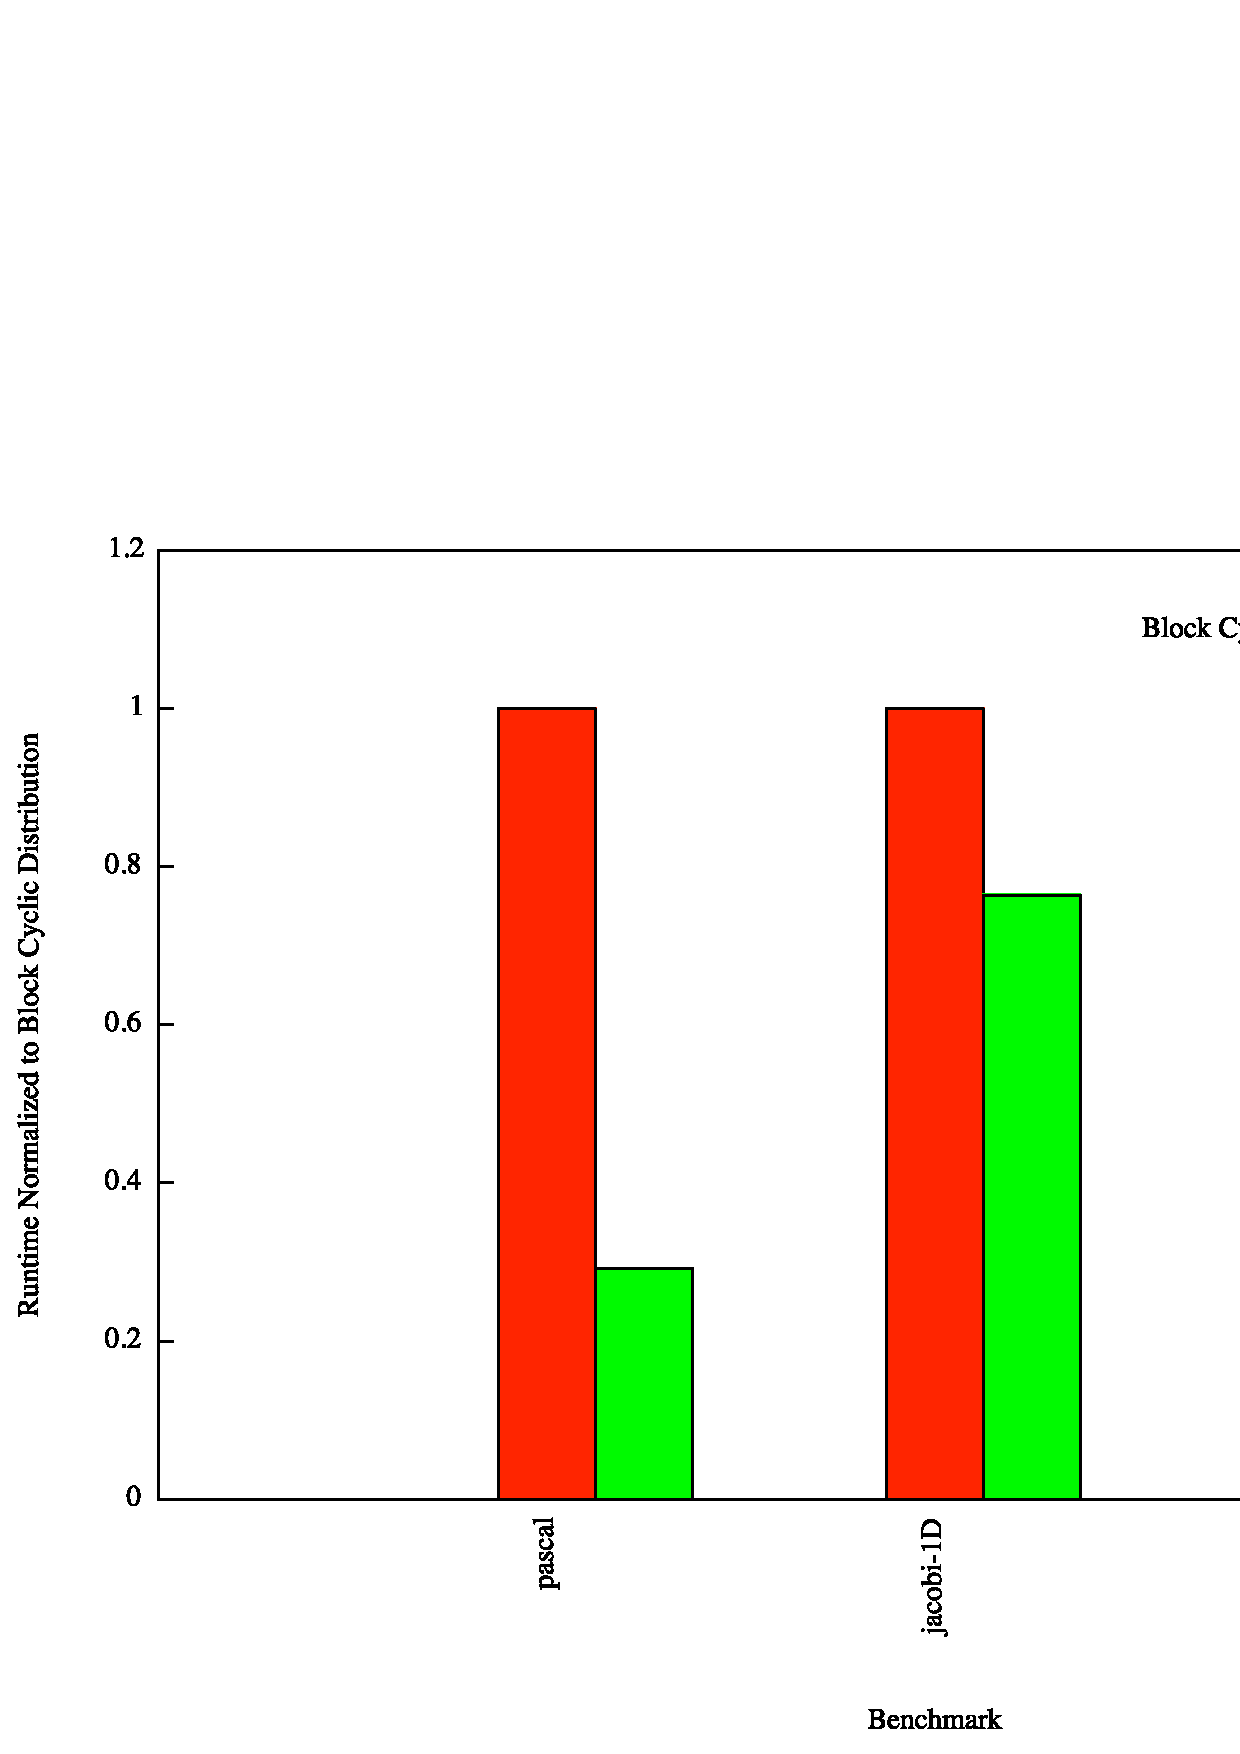
\includegraphics[scale=0.30]{./Figures/block_cyclic_runtime}
\caption{Block Cyclic runtime.}
\label{block_cyclic_runtime}
\end{center}
\end{figure}

\begin{figure}
\begin{center}
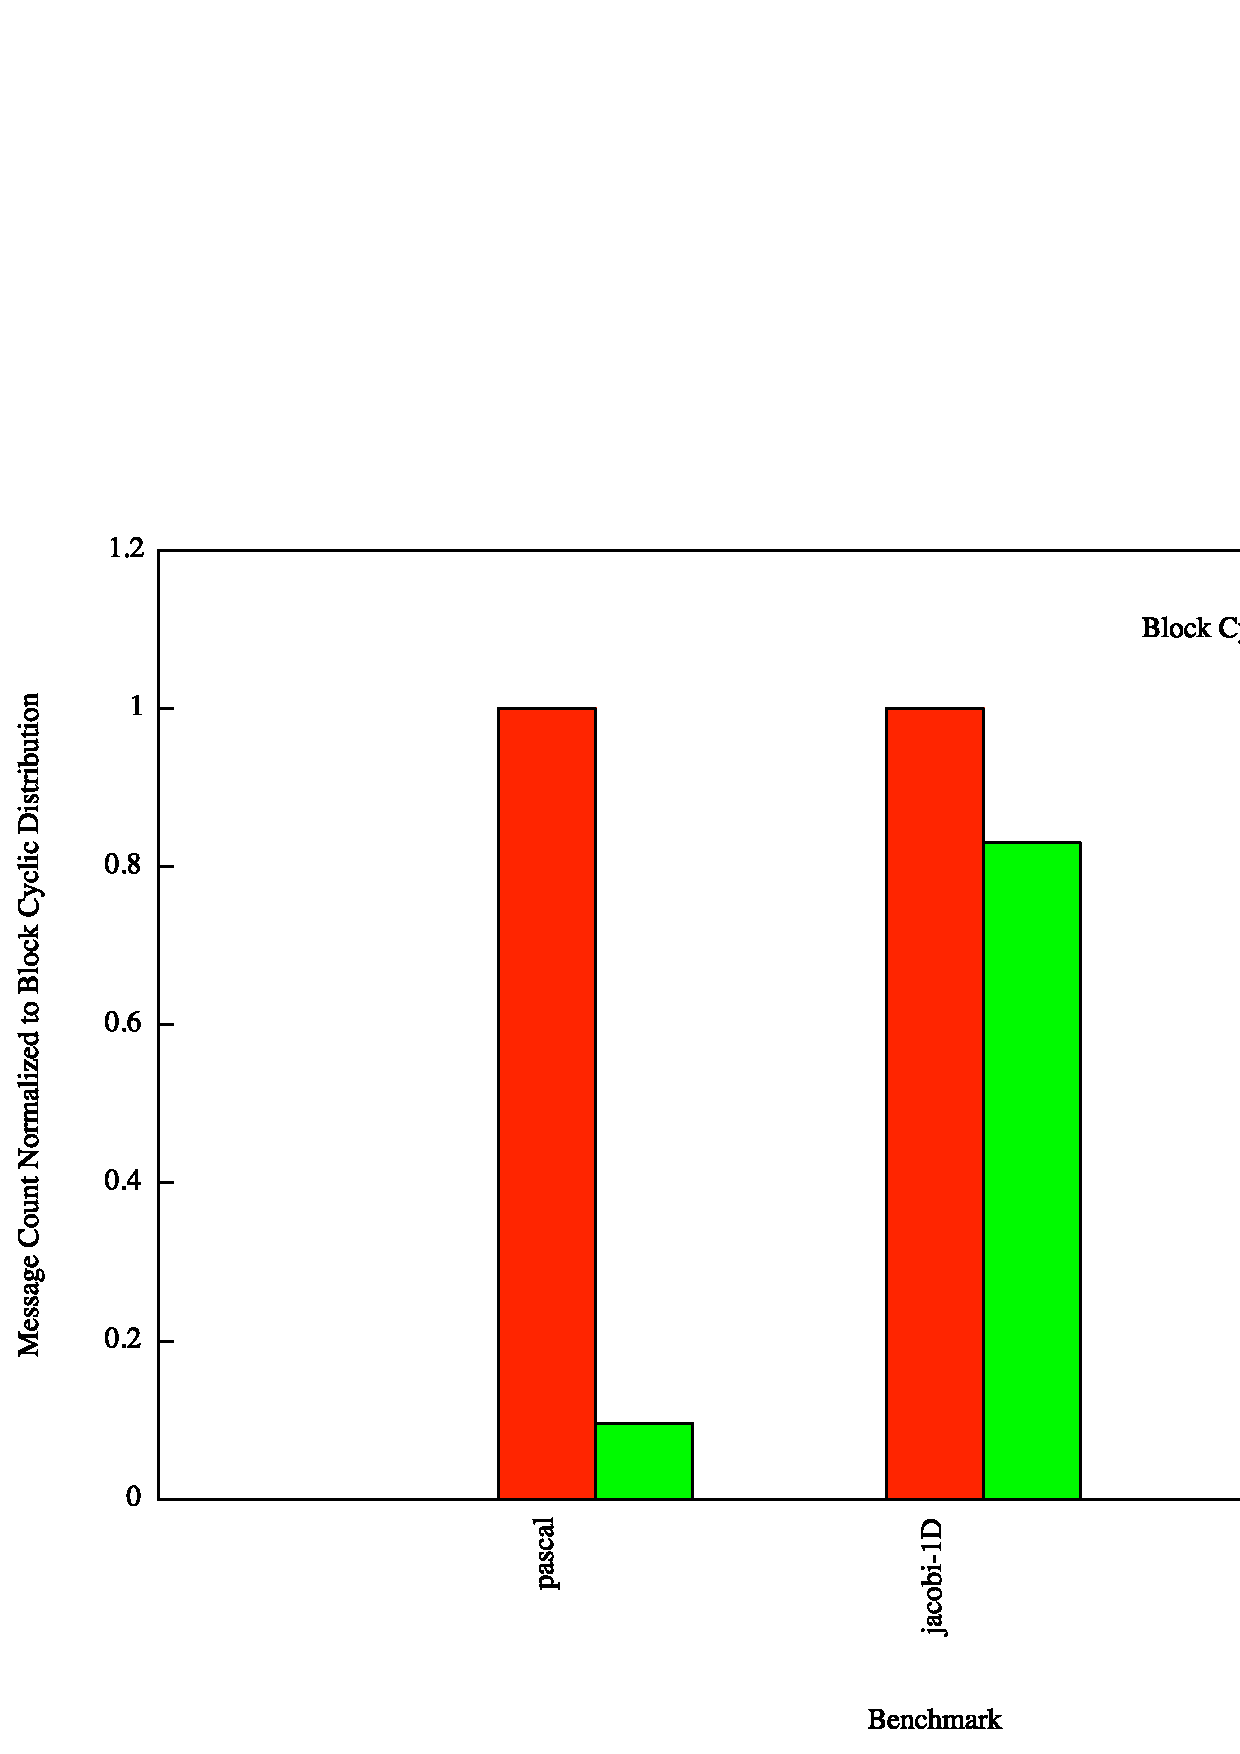
\includegraphics[scale=0.30]{./Figures/block_cyclic_message_count}
\caption{Block Cyclic message count.}
\label{block_cyclic_message_count}
\end{center}
\end{figure}

Figures \ref{block_cyclic_runtime} and \ref{block_cyclic_message_count} compare the normalized runtimes and message counts respectively for the Block Cyclic distribution and Block Cyclic distribution with modulo unrolling WU. For both benchmarks, we see reductions in runtime when the modulo unrolling WU optimization is applied. On average, modulo unrolling WU results in a 52 percent decrease in runtime. For both benchmarks, we see reductions in message counts when the modulo unrolling WU optimization is applied. On average, modulo unrolling WU results in 72 percent fewer messages. 